\section{Parámetros del refinamiento utilizando \ac{RDT}}
\label{anexo:criterios}


\begin{figure}[h]
   \centering
    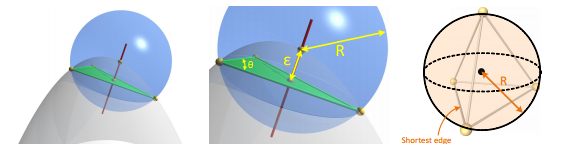
\includegraphics[width=0.8\textwidth]{IMG/rdt.png}
     \caption{Triangulación Restringida de Delaunay (\acs{RDT}). A la izquierda, faceta superficial con esfera de \emph{Delunay}. En el centro, detalle de los criterios utilizados para el refinamiento. A la derecha, \emph{circunsfera} asociada a un tetraedro.}
\label{fig:rdt}
\end{figure}


La \ac{RDT} es un algoritmo iterativo que genera una malla de tetraedros atendiendo a una serie de criterios de tamaño y forma. En primer lugar se definen una serie de elementos geométricos sobre los cuales se comprueban las restricciones (figura \ref{fig:rdt}).

\begin{itemize}
    \item Faceta superficial: Faceta de un tetraedro que aproxima la superficie del dominio
    \item Esfera de \emph{Delaunay}: Esfera de radio mínimo con centro en la superficie del dominio y que contiene a la faceta superficial
    \item \emph{Circumsfera} (asociada al tetraedro): Esfera de radio mínimo que contiene los cuatro vértices de un tetraedro
\end{itemize}




Las restricciones sobre las facetas superficiales son las siguientes:
\begin{itemize}
    \item  Tamaño: Radio máximo de la esfera de \emph{Delaunay}
    \item Forma: Límite inferior para los ángulos de la faceta superficial
    \item Aproximación: Distancia máxima entre la faceta superficial y el centro de la esfera de \emph{Delaunay}

\end{itemize}

Las restricciones sobre los tetraedros son las siguientes:
\begin{itemize}
    \item Tamaño: Radio máximo de la \emph{circumsfera}
    \item Forma: Relación máxima entre el \emph{circumradio} y la arista mas corta del tetraedro
\end{itemize}



Gracias a estos criterios, es posible controlar tanto la aproximación de la malla de tetraedros a la superficie como el tamaño general de tetraedros y triángulos, consiguiendo así reducir el número de tetraedros en las zonas donde no hacen falta y aumentando la resolución allí donde se requiera una mejor aproximación.
